\subsection{Kontextdiagramm}
-MJ-


Zu Beginn des Systementwurfs wurde ein Kontextdiagramm erstellt( siehe Abb. \ref{fig:context}). Das Kontextdiagramm dient zur Modellierung der Systemumgebung bildet die Schnittstellen zur Umwelt ab. So soll der Rettungsroboter z.B. eine Gegensprechanlage besitzen, um eine verbale Kommunikation zwischen dem Rettungsdienst und der zu rettenden Person zu ermöglichen. Außerdem wurden im Kontextdiagramm noch weitere Anforderungen spezifiziert. So soll die Hinderniserkennung mit Ultraschallsensoren umgesetzt werden.

\begin{figure}[h]
    \centering
    \captionsetup{width=.9\linewidth}
    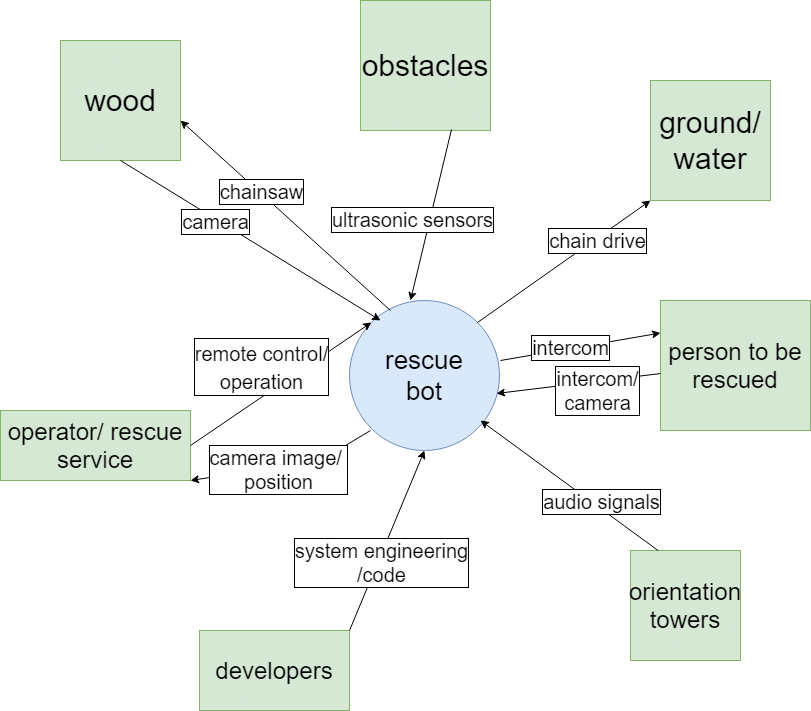
\includegraphics[width=1\linewidth]{contex_diagram.png}
    \caption{Kontextdiagramm}
    \label{fig:context}
\end{figure}